\documentclass[]{article}
\usepackage[top=1in,bottom=1in,left=1in,right=1in]{geometry}
\usepackage{amsmath}
\usepackage{graphicx}
\usepackage{natbib}

\begin{document}

\title{SPHERICAL/ASTRONOMICAL COORDINATE TRANSFORMATION}
\author{Carl Heiles and Deepthi Gorthi\footnote{Only translation to Python commands}}

\maketitle

    In our never-ending attempt to make your life easier, we present
you with the quickest of quick summaries of spherical coordinate
transformation with matrix techniques.  For example, you might need to
point the telescope at some particular position in the Galaxy.  In other
words, you need to convert from Galactic coordinates to altitude and
azimuth.  This involves three separate coordinate transformations:
Galactic longitude and latitude to equatorial right ascension and
declination [$(\ell, b) \rightarrow (\alpha, \delta)$]; to hour angle
and declination [$(\alpha, \delta) \rightarrow (ha, \delta)$]; to
azimuth and altitude [$(ha, \delta) \rightarrow (az, alt)$].  Or maybe
you need to go all or partway in the the other direction, i.e.  [$(az,
alt) \rightarrow [(\alpha, \delta)$] or maybe just [$(az, alt)
\rightarrow [(ha, \delta)$]. 

    These are conversions among four spherical coordinate systems. 
Such conversions involve all those complicated combinations of trig
functions (sigh).  You can write down all these trig functions for the
various possible transformation---twelve possibilities in all if you
include going both directions. 

    But there is a much easier, more elegant, and more politically
correct way: using {\it rotation matrices}.   In this method, you
generate a vector in the original coordinate system; convert the vector
to another coordinate system by rotating the coordinates using matrix
multiplication; and convert the vector to the angles of the new
coordinate system.  

    There are two big advantages with this method.  First, you can
apply several transformations in succession by multiplying the rotation
matrices in succession, so you break the process down into single
transformations, each with its own rotation matrix.  Second, it's easy
to go ``backwards''---you just use the inverse of the matrix. 

    The method is {\it general} and can be applied to {\it any}
coordinate transformation.  Spherical coordinates are characterized by
two angles.  One ``goes around the $z$-axis''---it is like longitude on
the earth.  The other ``goes up and down'' and is like latitude on the
earth.  These angles are ``longitude-like'' and ``latitude-like'', and
we'll denote them by $long$ and $lat$.  Thus, for Galactic coordinates,
$\ell$ is the ``longitude-like'' $long$ and $b$ is the ``latitude-like''
$lat$; for equatorial coordinates, it's $\alpha$ (or $ha$) and $\delta$;
for terrestrial coordinates, it's $az$ and $alt$. 

    One more thing before we get into details. Our discussion is
oriented towards astronomy, but the method works for any type of
spherical coordinate transformation. There is an excellent, short
discussion of the general situation in Goldstein's {\it Classical
Mechanics}, \S 4.4.
% ARP: can now get this text on the web/wikipedia

\section {ROTATION MATRICES: THE METHOD}

    To restate the problem: we start with $(long, lat)$ in one
coordinate system and want to convert to $(long^\prime, lat^\prime)$ in some other
coordinate system. Here's the prescription:

    {\it Step 1.} First, convert the angles to rectangular
coordinates.  One would usually call these $(x, y, z)$; here, to
emphasize the vector/matrix flavor, we call them $(x_0, x_1, x_2)$ and
denote the 3-element vector ${\vec x}$.  To accomplish this conversion:

\begin{align}
x_0 &= \cos(lat) \cos(long) \; , \\
x_1 &= \cos(lat) \sin(long) \; , \\
x_2 &= \sin(lat) \; .
\end{align}

\noindent The Python/NumPy commands to accomplish this should be obvious, so we
won't state them here; but remember to convert the arguments to radians
(converting degrees to radians is most easily done by using 
{\tt np.radians(angle)}). 

    {\it Step 2.} Apply the rotation matrix ${R}$ (we'll discuss its
definitions below): 

\begin{equation}
{\vec x^\prime} = {R \cdot x} \; .
\end{equation}

\noindent In Python, we'll use the Python variable ${\vec xp}$ to represent ${\vec
x^\prime}$, and you do matrix multiplication with the function {\tt np.dot(mat1,mat2)}\dots

\begin{equation}
{\vec xp} = np.dot(R,{\vec x}) \; .
\end{equation}

    {\it Step 3.} Convert the primed rectangular coordinates to the
new set of spherical coordinates $(long^\prime, lat^\prime)$:

\begin{align} 
long^\prime &= \tan^{-1} \left({{\vec x^\prime}_1 \over {\vec x^\prime}_0}\right) \; , \\ 
lat^\prime &=
\sin^{-1} ({\vec x^\prime}_2) \; .  
\end{align}

\noindent To do these in Python, where we'll write {\bf longp, latp}:

\begin{equation}
{ longp = np.arctan2(xp(1), xp(0))}
\end{equation}
\begin{equation}
{ latp = np.arcsin(xp(2))} \; ;
\end{equation}

\noindent if you want to convert their outputs to degrees, use the function
{\tt np.degrees(angle)}.  {\it IMPORTANT:} writing {\tt np.arctan2(xp(1), xp(0))} 
instead of {\tt np.arctan(xp(1)/xp(0))} ensures that the angle is given in the correct
quadrant.  See the Python documentation. 

    That's it! If you want to ``go backwards'', you just apply the
matrix multiplications using the inverse matrices.  For rotation
matrices, the inverse is always equal to the transpose(!)\footnote{If
you don't believe this, check on the ${R}$'s below in \S
2!}---symbolically for the matrix ${R}$, ${R^{-1}} = {R^T}$. 
So to go from the primed system to the unprimed, you switch the primed
and unprimed in equation (2) and use the inverse rotation matrix

\begin{equation}
{\vec x} = {R^{-1} \cdot x^\prime} = {R^T \cdot x^\prime}\; .
\end{equation}

\noindent and in Python\dots

\begin{equation} 
{\vec x} = np.dot({\tt np.transpose(R)},{\vec xp})  
\end{equation}

\section {ROTATION MATRICES: SPECIFICS FOR OUR PROBLEM}

    OK, what are these rotation matrices? We'll do you a big favor
and tell you.  

\subsection {(RA, DEC) to (HA, DEC)---any epoch.}

    Converting from $(\alpha, \delta) \rightarrow (ha, \delta)$
keeps the declination the same and uses the relationship $ha = LST -
\alpha$.  It is easiest to think of this in two steps, so we express

\begin{equation} 
{R}_{(\alpha, \delta) \rightarrow (ha, \delta)} = 
{R}_{(\alpha, \delta) \rightarrow (ha, \delta), 2} \cdot 
{R}_{(\alpha, \delta) \rightarrow (ha, \delta), 1} \; .
\end{equation} 

\noindent First, we rotate around the equatorial pole by an angle equal
to the Local Sidereal Time ($LST$), which does $\alpha \rightarrow
(\alpha - LST)$:

\begin{eqnarray} 
{R}_{(\alpha, \delta) \rightarrow (ha, \delta),1} = \left[ 
\begin{array}{ccc} 
    \cos(LST) & \sin(LST) &  0 \\
   -\sin(LST) & \cos(LST) &  0 \\
            0 &  0        &  1 \\
\end{array} 
\; \right] \; .
\end{eqnarray} 

\noindent Next, the $ha$ and $\alpha$ go in opposite directions, which
is equivalent to converting from the original left-handed to a
right-handed coordinate system, so the second step is just to perform
this reversal:

\begin{eqnarray} 
{R}_{(\alpha, \delta) \rightarrow (ha, \delta), 2}  = \left[
\begin{array}{ccc}
    1 & 0 &  0 \\
    0 & -1&  0 \\
    0 &  0&  1 \\
\end{array} 
\; \right] \; .
\end{eqnarray} 

\noindent The full rotation matrix is the matrix product ${
R}_{(\alpha, \delta) \rightarrow (ha, \delta),2} { \cdot} {
R}_{(\alpha, \delta) \rightarrow (ha, \delta), 1}$.  {\it Note the
order!} Applying ${R}_{(\alpha, \delta) \rightarrow (ha, \delta),2}$
at the {\it beginning} in the matrix product means that it operates {\it
last} on the vector ${\vec x}$, which is what we want.  So we have as the
product\dots

\begin{eqnarray} 
{R}_{(\alpha, \delta) \rightarrow (ha, \delta)} = \left[ 
\begin{array}{ccc} 
    \cos(LST) & \sin(LST) &  0 \\
    \sin(LST) & -\cos(LST) &  0 \\
            0 &  0        &  1 \\
\end{array} 
\; \right] \; .
\end{eqnarray} 

\subsection {(HA, DEC) to (AZIMUTH, ALTITUDE).}

    Because $(ha, \delta)$ are Earth-based coordinates, this
conversion depends only on your terrestrial latitude $\phi$:

\begin{eqnarray} 
{R}_{(ha, \delta) \rightarrow (az, alt)} = \left[ 
\begin{array}{ccc} 
-\sin \phi &    0    & \cos \phi \\ 
      0    &   -1    &    0      \\ 
 \cos \phi &    0    & \sin \phi \\ 
\end{array} 
\; \right] \; .
\end{eqnarray} 

\subsection {EQUATORIAL to GALACTIC.}

\begin{eqnarray} 
{R}_{(\alpha, \delta)_{1950} \rightarrow (\ell, b)} = \left[ 
\begin{array}{rrr}
   -0.066989 &  -0.872756 &  -0.483539 \\
    0.492728 &  -0.450347 &   0.744585 \\
   -0.867601 &  -0.188375 &   0.460200 \\
 \end{array} 
\; \right] \; .
\end{eqnarray} 

\noindent This is from Green's {\it Spherical Astronomy}, chapter 14.6,
problem 14.6 (answers in back of book).  We should've made you derive
this, but we're softies.  You {\it really should} at least {\it glance}
at Green's chapter 2.7, which defines Galactic coordinates.  In truth,
the precession of the equatorial coordinate system makes this matrix a
function of time: the equatorial coordinates move around the sky, but
the Galactic ones do not.  Precession amounts to nearly an arcminute per
year! In principle, you should derive the matrix for the current epoch. 
In practice, you may not need such high accuracy.  Better than the 1950
version are the numbers for epoch 2000, which are in Green's equation
(14.55); epoch 2000 is lots closer to the present than is epoch 1950:

\begin{eqnarray} 
{R}_{(\alpha, \delta)_{2000} \rightarrow (\ell, b)} = \left[ 
\begin{array}{rrr}
   -0.054876 &  -0.873437 &  -0.483835 \\
    0.494109 &  -0.444830 &   0.746982 \\
   -0.867666 &  -0.198076 &   0.455984 \\
\end{array} 
\; \right] \; .
\end{eqnarray} 

\subsection {Precession---converting equatorial between epochs.}

    We won't need these for the lab course, but we give you the info
for the sake of completeness.  Generating the rotation matrix for
precession is a bit tedious and we won't give the explicit formulae
here.  They are in Green's book.  The elements of the matrix are in
equation (9.31).  These elements contain angles, which depend on time as
in equation (9.23) if you are converting from epoch 2000 to some other
epoch.  Precession isn't all there is; for precision exceeding $\sim
10''$ you also need to account for nutation of the Earth, which has a
random component and is not completely predictable.  For the complete
story, see Green's chapter 9 and {\it The Astronomical Almanac 1998}, 
pages B39-B43---for interested parties only!

\paragraph{Note on Angle Representations}
Angles are usually specified in degrees or radians with decimal places 
representing the fractional angle. In astronomy, you will often encounter 
angles represented in degrees, minutes and seconds. You can convert this into 
decimal degrees ($dd$) using the fact that there are 60 minutes in a degree and 60 seconds in a minute.

\begin{equation}\label{eq:dd2dms}
dd = \text{degree} + \text{minutes}/60 + \text{seconds}/3600
\end{equation}

You will also often encounter the sexagesimal notation where angles are represented in hours, minutes and seconds. This is especially useful to represent angles that are dependent on longitude of the location since $15^\circ$ is equivalent to an hour. You can convert a sexagesimal angle to decimal degrees using equation (\ref{eq:dd2dms}) and the additional multiplying factor of $15^\circ$. 

\section {DOING ALL THIS IN Python}

    Obviously, all this stuff is simple in Python, which deals easily with
matrices:

%\subsection {A CRUCIAL PRELIMINARY: 2-D arrays in IDL.}
%
%    In a computer, a multidimensional data set can be indexed in two
%ways, the {\it column-major} and {\it row-major} formats.  IDL uses the
%row-major format, as does Fortran; the other major language, C, uses
%column-major.  Suppose you have a $2 \times 2$ matrix called ${ A}$. 
%In IDL's row-major format, when you type [{\it print, A}] IDL prints
%
%\begin{eqnarray} 
%\left[ 
%\begin{array}{rrr}
%A_{0,0} & A_{1,0} \\
%A_{0,1} & A_{1,1} \\
%\end{array} 
%\; \right] \; ,
%\end{eqnarray} 
%
%\noindent which is different from what you are used to seeing in
%standard matrix notation which is the column-major format
%\begin{eqnarray} 
%\left[ 
%\begin{array}{rrr}
%A_{0,0} & A_{0,1} \\
%A_{1,0} & A_{1,1} \\
%\end{array} 
%\; \right] \; .
%\end{eqnarray} 
%    In this writeup, we are defining matrices such that, when
%displayed in a standard IDL {\it print} statement, they look correct.
%For example, in equation (12b), the upper right-hand element $-0.483835$
%is $R_{2,0}$. 
%
%    If you want to be a purist and define the matrices in the
%standard manner, that is with the lower left-hand element $-0.483835$
%being $R_{0,2}$ instead of $R_{2,0}$, go ahead and do so.  You then need
%to do two things.  First, if you want to see the matrix displayed in the
%usual way, then print its transpose by typing [{\it print,
%transpose(A)}].  Second, in all our IDL matrix equations, replace ${
%\# \#}$ by ${ \#}$. 
%
%    Why does IDL do this nonstandard thing? It's because it's more
%straightforward for image processing, in which traditionally the images
%are scanned row-by-row (as in a TV set) instead of column-by-column. And
%IDL's origins are image processing, not matrix math.

\subsection {Try the following examples in Python.}

Test ${R}_{(ha, \delta) \rightarrow (az, alt)}$, going both forwards
and backwards. For an observatory at latitude $41.36^\circ$,
$(az,alt)=(137.60^\circ,32.43^\circ)$ transforms to
$(ha,\delta)=(325.05s^\circ, -6.52^\circ)$.  Hour angle is usually given
in hours using sexagesimal notation: $ha=21^h40^m12^{s}$.) 

%See the IDL
%functions {\tt sixty} and {\tt ten} to go back and forth between decimal
%and sexagesimal notations.

    Test ${R}_{(\alpha, \delta) \rightarrow (ha, \delta)}$ by
making up your own example, using the fact that $ha = LST - \alpha$. 

    Test ${R}_{(\alpha, \delta)_{1950} \rightarrow (\ell, b)}$
for the Crab Nebula. The Crab has 1950
equatorial coordinates $(\alpha, \delta)=(05^h31^m.5, 21^\circ59')$ and
Galactic coordinates $(\ell,b)=(184^\circ33', -5^\circ47')$.

%\enlargethispage*{0.5in}
    Finally, put them all together and make sure that works, too. 
For {\it all} of these, make sure you know how to go backwards! For
example, suppose you want to convert $(az, alt) \rightarrow (\alpha,
\delta)$.  You need to first apply ${R}_{(ha, \delta) \rightarrow
(az, alt)}^{-1}$ and then ${R}_{(\alpha, \delta) \rightarrow (ha,
\delta)}^{-1}$.  So the full rotation matrix in this case is\dots
\begin{equation}
{R}_{(az, alt) \rightarrow (\alpha, \delta)} = 
{R}_{(\alpha, \delta) \rightarrow (ha, \delta)}^{-1} \cdot
{R}_{(ha, \delta) \rightarrow (az, alt)}^{-1}
\end{equation}
\noindent Again, {\it note the order!} Applying ${R}_{(\alpha,
\delta) \rightarrow (ha, \delta)}^{-1}$ at the {\it beginning} in the
matrix product means that it operates {\it last} on the vector ${\vec x}$. 

%\begin{figure}
%\includegraphics[width=7.0in] {page107.ps}
%\end{figure}  
%
%\begin{figure}
%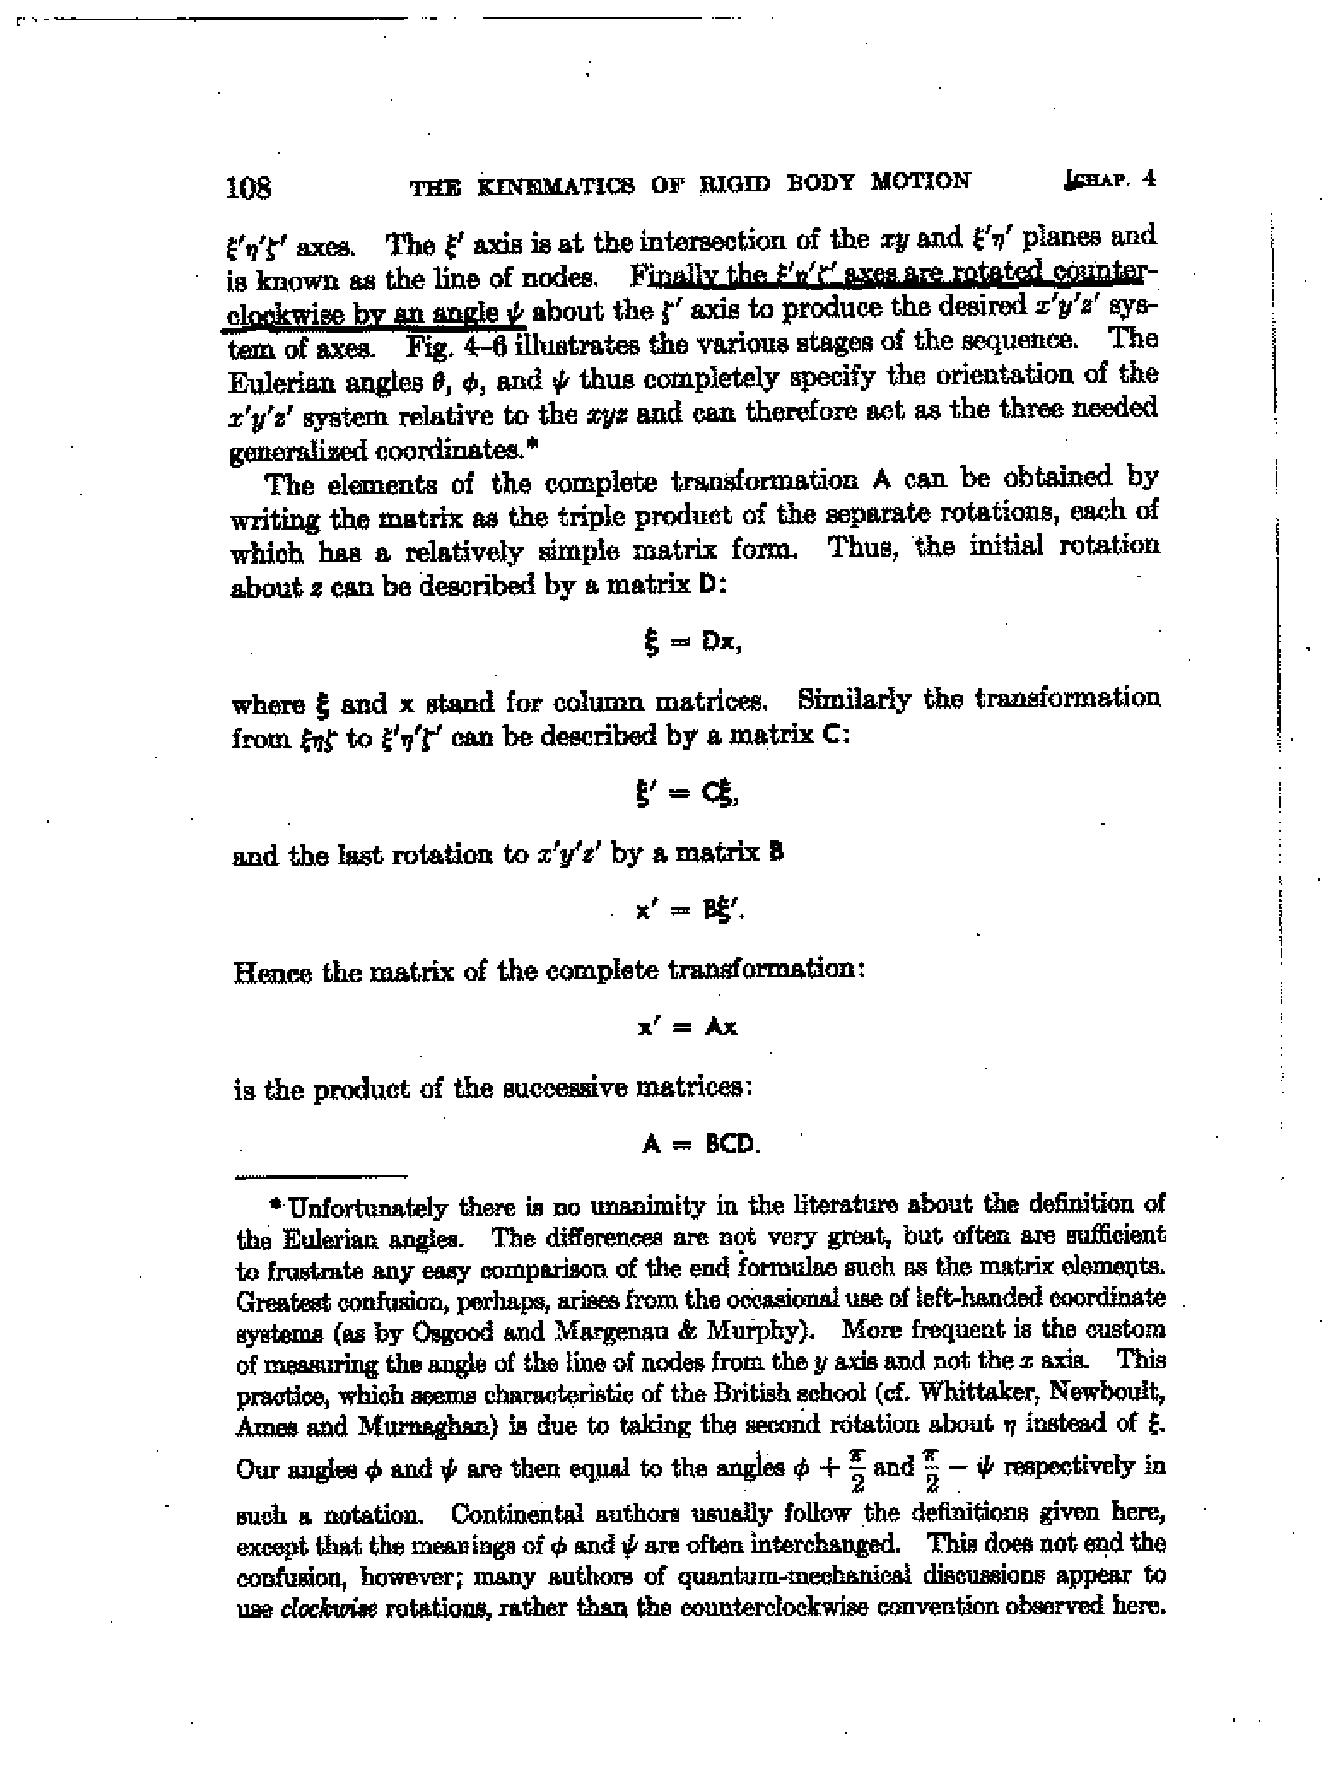
\includegraphics[width=7.0in] {page108.ps}
%\end{figure}  
%
%\begin{figure}
%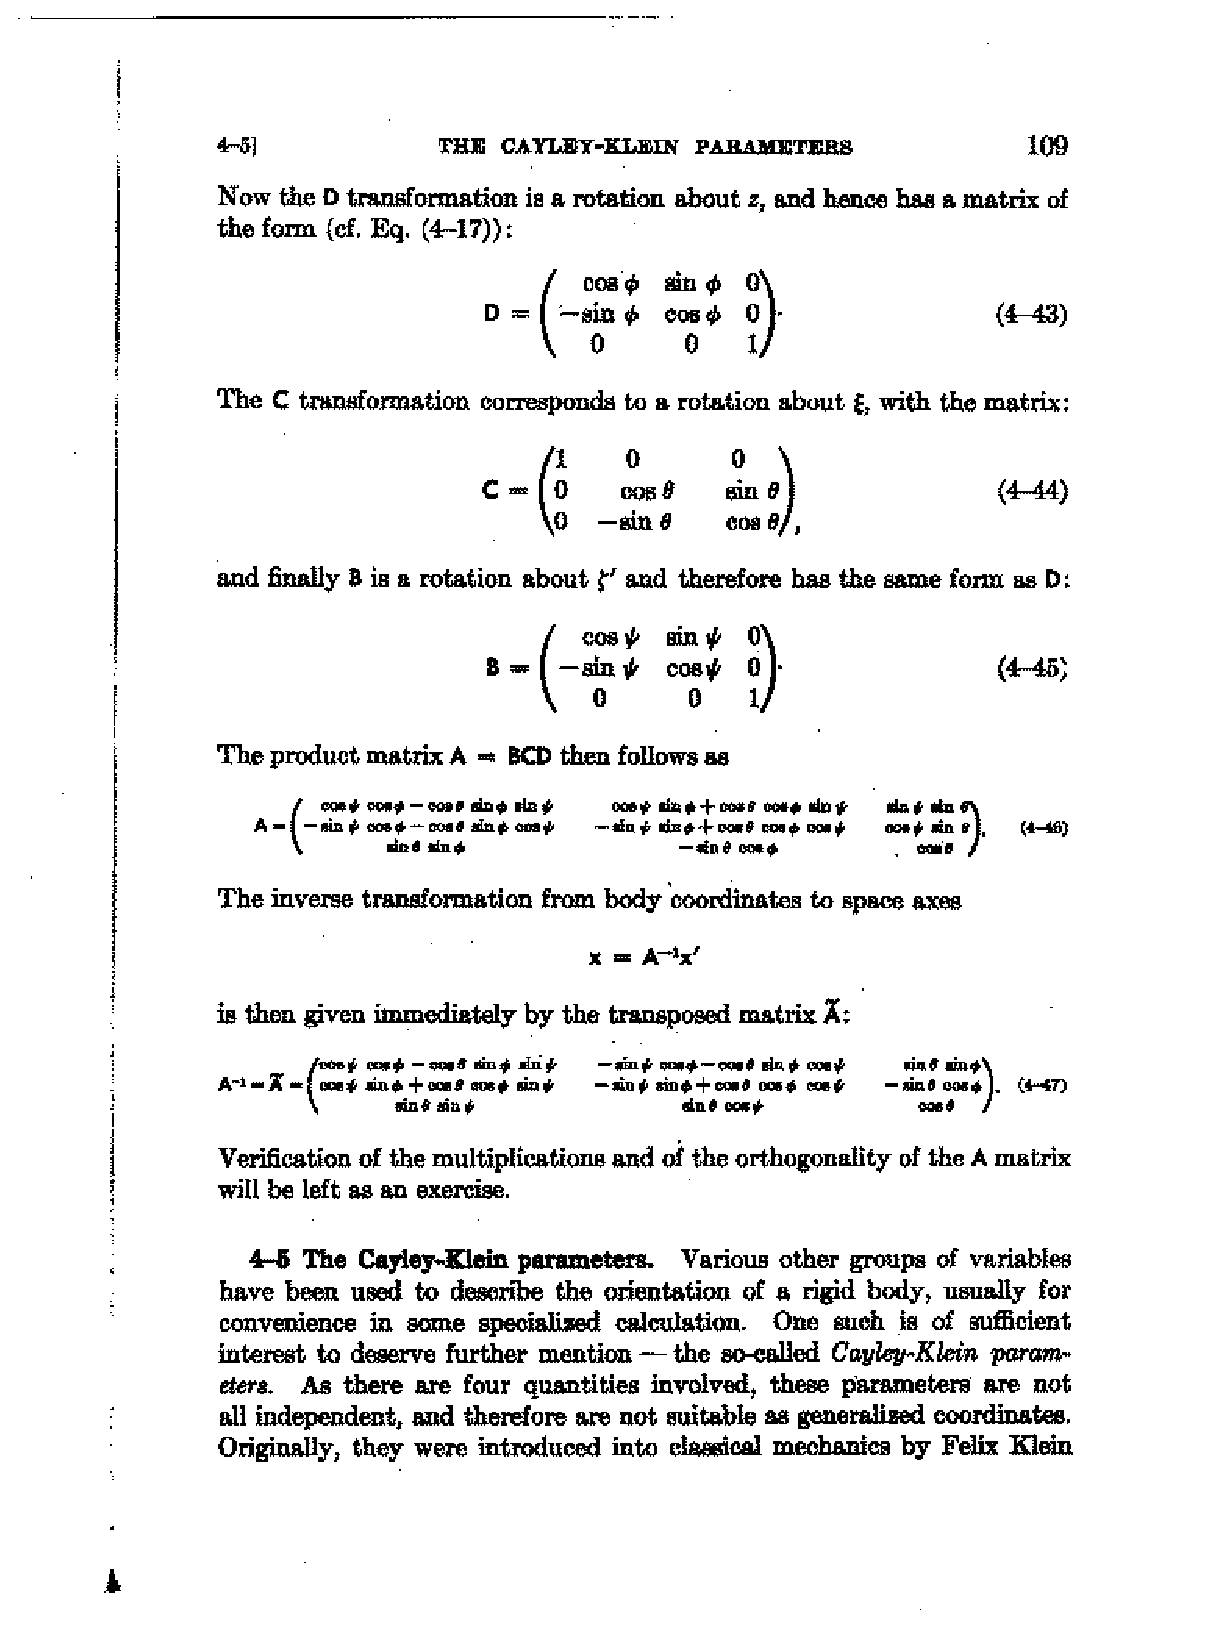
\includegraphics[width=7.0in] {page109.ps}
%\end{figure}  

\end{document}
